% ================================================================= QUEUE ==
\section{Task 2: queue forecasting}\label{sec:queue}

\subsection{Formulation}
A window $w$ has origin $T$ and history $H_w$: speed, flow, occupancy, eligibility and ramp counts on the twelve slots
$T{-}60,\dots,T{-}5$ (\cref{fig:t2window}). We must output a binary field $a\in\{0,1\}^{6\times L}$ over links and the
six horizons. The decision that maximizes the expected score is
\begin{equation}
  a^\star(H_w) = \arg\max_{a}\ \mathbb E\big[\IoU(a,Y)\,\big|\,H_w\big],
  \label{eq:bayes}
\end{equation}
which has no closed form because IoU is a ratio over the whole field \cite{nowozin2014}. We approximate the
expectation in two ways. An \emph{empirical} estimate averages the IoU of $a$ against the complete outcomes $y_j$ of
analogous training windows \cite{lorenz1969}. A \emph{model} estimate uses per-cell probabilities $p_i$ and the ratio of
expected intersection to expected union,
\begin{equation}
  \widehat{\IoU}_p(a) = \frac{\sum_i a_i p_i}{\sum_i a_i + \sum_i p_i - \sum_i a_i p_i}.
  \label{eq:modeliou}
\end{equation}
This ratio of expectations is not the exact expected IoU, but it rewards the right trade-off between size and
confidence, which a per-cell threshold does not.

\subsection{What the window selection implies}
Two properties of the selector (\cref{sec:design}) decide the shape of a good forecaster.
\begin{itemize}
  \item \textbf{Onset queues appear at the last step.} In the 40 published training onset windows the median first
        crossing of $0.6\,v_f$ is at horizon 6. The head of the queue is usually a recurrent bottleneck whose location
        a training prior already contains: the top three links of a frequency prior include it in 79\,\% of events. The
        size is the hard part. With a perfect head and an unknown extent a contiguous block scores about 0.62 latent IoU;
        with the true extent, 0.905. Extent varies from one to eight links and we found nothing in the legal hour that
        predicts it (correlation 0.05 with daily demand, 0.10 with hourly demand).
  \item \textbf{Ongoing windows are those persistence gets wrong.} Windows with persistence IoU above 0.9 are excluded.
        In 31 of the 40 published ongoing windows the queue began before $T{-}60$, so most queues are mature, and their
        evolution over the next 30 minutes (clear, hold or grow) is the forecast.
\end{itemize}

\subsection{Ongoing queues: start by not dropping sensors}\label{sec:ongoing}
The organizer's persistence baseline repeats the queue state of slot $T{-}5$ using eligible cells only. Between 23 and
24\,\% of links have a missing or ineligible $T{-}5$ reading in every split, and persistence then predicts ``not
queued'' there. Forward-filling the last \emph{released} value of each link over the twelve slots, ineligible readings
included, keeps those links. On the public board this raised ongoing IoU from about 0.603 to 0.738 (U2 against U1,
an ongoing-only change of +0.02021 in total). A diagnostic that set ongoing queues from the state at slot $T$
(P-slotT) reached only about 0.729. On the training windows slot $T$ adds $+0.003\pm0.002$ latent IoU over the legal
forward-fill: what mattered was not the extra slot but not throwing away the sensors that were already there.

\subsection{Onset: a joint-mask analogue}\label{sec:onset}
Per-link classifiers decide each link independently and so cannot represent the joint size and shape of an onset.
The J1 rule instead chooses a complete mask from the outcomes of similar training events.
\begin{enumerate}
  \item \textbf{Event pool.} Training origins that meet the legal onset definition (no queue in $T{-}60\dots T{+}25$,
        a queue at $T{+}30$, history coverage at least 0.7), within $\pm30$ minutes of the query origin. Candidates are
        tiered: same day type (weekday or weekend) and local time first, then any day type, then any slot.
  \item \textbf{Similarity.} Thirteen descriptors of the legal hour: total flow over capacity (last, mean, change), the
        mean speed-to-threshold ratio (last, mean, change), the minimum ratio, the eligibility rate, total ramp flow
        (last, mean, change), and the sine and cosine of the time of day. Distance is the standardized RMS difference,
        and the ten nearest events are kept.
  \item \textbf{Action set.} Each neighbour's observed $T{+}30$ mask, plus the top-$k$ links of the neighbours' marginal
        frequency for $k=1,\dots,15$.
  \item \textbf{Bayes action.} The action with the highest mean IoU against the ten neighbour outcomes on their known
        cells, placed at $T{+}30$ only; horizons 1--5 are empty.
\end{enumerate}
In public, the legal LightGBM onset classifier scored about 0.626 IoU, a frequency prior 0.450 and J1 0.750
(\cref{tab:components}). J1 has been the onset of every candidate since, including both selected files. Its 0.75 is
close to what the training analysis says twelve slots allow (0.62 with unknown extent, 0.905 with the true extent).

\subsection{Ongoing queues: classifier, analogue library and decoder}\label{sec:decoder}
\paragraph{Training population} A training origin is \emph{difficult} when its observed six-step future has queued
cells, its denoised origin state has a queue, and six-step persistence scores at most 0.9 IoU on it, mirroring the
selector. A \emph{first crossing} is a difficult origin whose predecessor was not difficult. Q46 was fitted on 2,093
first crossings from July--November (at most 300 per panel). EQ1, in ES4, keeps every one of them and adds up to 240
date-diverse first crossings per panel from June, December, January and February: 3,766 windows and 3,172,453 rows.
Future training observations are labels only, never inputs.

\paragraph{Features} 213 inputs per link and horizon, all from the twelve legal slots (\cref{tab:queue-features}).
Beyond lags and summaries, two groups carry the traffic physics. Distance bands summarize the speed ratio, flow ratio
and density 1, 2, 4, 8 and 16 km upstream and downstream. Characteristic features read the state along the free-flow
and backward-wave characteristics through each link, at ages of 0, 15 and 30 minutes, which is where a wave that will
reach the link within the horizon is visible now.

\begin{table}[h]
\centering\small
\caption{The 213 inputs of the ongoing-queue classifier.}\label{tab:queue-features}
\begin{tabularx}{\linewidth}{@{}l X r@{}}
\toprule
Group & Features & Count \\
\midrule
Lags & speed and flow at lags 1, 2, 3, 4, 6, 9, 12 slots & 14 \\
Summaries & recent, previous, early, min, max, std, slope, trend, coverage, age; for speed and flow & 20 \\
Neighbours & last value and trend at links $\pm1,\pm2,\pm4$; for speed and flow & 24 \\
Corridor & corridor mean, minimum and trend; for speed and flow & 6 \\
Queue context & queued neighbours at $\pm1,\pm2,\pm3$, queued count and its change, nearest queue up- and downstream & 10 \\
Density & $q/v$ density, last value, trend, acceleration, distance to the queue cut & 5 \\
Distance bands & speed ratio, flow ratio and density at $\pm1,2,4,8,16$ km: recent, trend, extreme & 90 \\
Characteristics & free-flow and wave characteristics, both directions, ages 0/3/6 slots; speed, flow, density & 36 \\
Static and calendar & free-flow speed, per-lane capacity, lanes, length, per-lane jam density; slot, weekend, horizon & 8 \\
\midrule
Total & & 213 \\
\bottomrule
\end{tabularx}
\end{table}

\paragraph{Classifier} A LightGBM binary model with 63 leaves and learning rate 0.05, equal weight per panel and per
window, and the horizon as an input, so one model covers all six steps. Q46 has 400 trees; EQ1 has 800.

\paragraph{Analogue library} Every training origin, at a stride of two slots, is encoded by its twelve-slot speed and
flow ratios and its complete six-step future. For a query, donors are restricted to $\pm2$ hours of time of day and the
same weekend flag when at least 20 such donors exist. The distance is the mean squared difference of the speed-ratio
history, with links currently below $0.85\,v_f$ weighted thirteen times, plus 0.4 times the flow-ratio distance, plus
0.15 times one minus the Jaccard overlap of the current queue sets. The 20 nearest donors are kept.

\paragraph{Candidate pool} The decoder chooses among at most 34 complete masks: the analogue's own choice; persistence;
the expected-count decoding of $p$; $p\ge0.4$ and $p\ge0.5$; the 20 donor futures; the donors' marginal frequency
thresholded at 0.25, 0.40, 0.55 and 0.70; the union and intersection of the analogue choice with the decoded $p$; and
the expected-count decoding of $\alpha\,\text{marginal}+(1-\alpha)\,p$ for $\alpha\in\{0.25,0.5,0.75\}$.

\paragraph{Decoder (RQ48)} With $\widehat{\IoU}_{\mathrm{emp}}(a)$ the mean IoU of $a$ against the donor futures on their
known cells, the deployed choice is
\begin{equation}
  \hat a = \arg\max_{a\in\mathcal A}\ \Big[\,0.25\,\widehat{\IoU}_{\mathrm{emp}}(a) + 0.75\,\widehat{\IoU}_p(a)\,\Big].
  \label{eq:rq48}
\end{equation}
The earlier rule used equal weights. Four weightings were registered before development; the quarter weight had
the largest minimum gain across the March and April development samples, passed its single confirmation
(+0.0335 and +0.0300 on even dates, date-clustered 95\,\% intervals [0.013, 0.054] and [0.012, 0.051]), and measured
+0.00469 in public, which corresponds to +0.031 ongoing IoU.

\subsection{Results and the selection gap}\label{sec:queue-results}
\Cref{tab:components} gives the public evidence. Ongoing IoU rose from about 0.603 (organizer persistence) to 0.738
(forward-fill) and 0.766 (first analogue decoder); two later steps changed the state as well and cannot be split, then
RQ48 added +0.031 and EQ1 +0.003. If the two state corrections in those mixed steps contributed between nothing and
their full held-out proxy value, ES4's ongoing IoU is between 0.827 and 0.832 in public. Onset stayed at 0.750.

\begin{figure}[t]
\centering
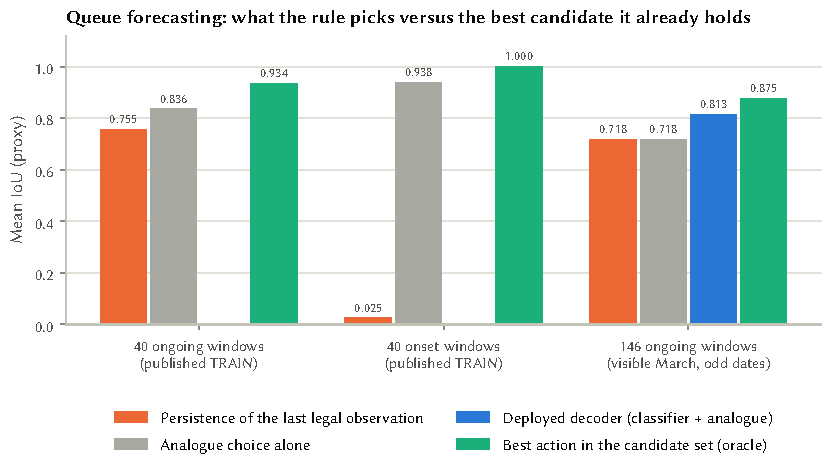
\includegraphics[width=\linewidth]{figures/fig_queue_ceiling.pdf}
\caption{The selection gap. ``Best action'' is the highest-scoring mask already in the candidate set, identified with
the label after the choice; it is a diagnostic, not a forecast. Published windows use latent labels; March windows
use visible observations. The full decoder was not scored on the June instrument.}\label{fig:queue-ceiling}
\end{figure}

\Cref{fig:queue-ceiling} shows where the remaining queue error lives. On the 40 published ongoing windows, the
analogue's choice scores 0.836 while the best mask in its own candidate set scores 0.934. On 146 visible March
windows the deployed decoder scores 0.813 against a best-in-set 0.875, and the analogue's choice alone ties
persistence (0.718). On 160 hard November windows the best whole-window action scores 0.946 and the best per-link
combination 0.967, against 0.807 for the deployed whole-window rule. The candidates are good enough; choosing among
them is not. None of the frozen selection rules we tried cleared its pre-set gain on held-out windows (0.02--0.03
IoU): a ridge reranker (+0.007), an expected-overlap-minus-disagreement ranker (+0.009), a cell majority of the 20
donors (+0.004), a neighbour-bit classifier ($-0.010$), per-link nearest-neighbour copies ($-0.022$), odd-date panel
weights and a March-fit reranker (\cref{sec:negative}).

\begin{keybox}[Insight]
Queue forecasting here is a decision problem over complete masks. The two largest gains came from keeping
information (forward-filling dropped sensors) and from respecting the joint structure of the outcome (choosing whole
onset masks by expected IoU). Better per-cell probabilities moved the score less than the choice among whole masks,
and that choice, not the candidate set, is where the remaining error sits.
\end{keybox}
